\chapter{Commande par modèle prédictif}
\label{chapitre.commande}
	\section{Principe}
	
		L'objectif de ce chapitre est de présenter la loi de commande permettant de réaliser les mouvements et l'équilibre d'un robot humanoïde à roues omnidirectionnelles.
		Dans le chapitre \rf{chapitre.modele}, nous avons développé un modèle du robot utilisant deux corps.
		Les contraintes de complémentarités dues aux forces de contact nous ont emmené à modéliser le robot en deux parties : lorsque celui-ci possède ses trois roues en contact avec le sol, et lorsqu'il bascule sur deux de ses roues.
		Ensuite de quoi, nous avons montré qu'il est important de modéliser la dynamique dans le futur à cause des contraintes sur le CoP, qui limitent fortement les mouvements réalisables par le robot.
		Enfin, deux équations prédictives de la dynamique ont été formulées :
		\liste{
			\item Dans le cas où le robot possède trois roues sur le sol, l'équation \rf{eq.dyn_cop_pred} exprime la relation entre la position du CoP et la dynamique des corps du robot.
			\item Dans le cas où le robot bascule sur deux roues, l'équation \rf{eq.dyn_tilt_pred} exprime la dynamique de l'angle de basculement en fonction de celle des corps du robot.
		}
		
		Nous avons donc choisi de réaliser une loi de commande optimale basée sur un modèle prédictif linéaire en les variables de commande, soumis à des contraintes linéaires.
		La fonction objectif de cette commande optimale est basée sur la minimisation d'une norme d'ordre $2$, permettant la convergence d'une grandeur d'erreur vers $0$, utilisés notamment dans une tâche de suivi de trajectoire.
		
		L'interêt de l'aspect prédictif de cette commande est de pouvoir utiliser les connaissances que l'on a sur le comportement dynamique du système ainsi que sur les mouvements demandés, pour prévoir et adapter en avance les trajectoires résultantes.
		Cela permet d'obtenir une meilleure réalisation des objectifs dans le temps. 
		Cette adaptation est nécessaire lorsque les contraintes du système réduisent de beaucoup l'ensemble des trajectoires atteignables instantanément par les corps du robot, ce qui est notre cas.
	
	\section{Outil mathématique et contraintes associées}
	
		Notre objectif est d'exécuter la loi de commande en temps réel sur la plate-forme expérimentale. 
		Il est donc important d'utiliser un outil mathématique de calcul qui permette cela.
		Le système étant fortement contraint (Position du CoP, limites articulaires, limites dynamique des moteurs), nous ne pouvons disposer d'une solution analytique.
		Une méthode de résolution numérique du problème doit donc être envisagée.
		
		Nous avons donc choisi d'utiliser la méthode de la programmation quadratique sous contraintes linéaires (QP).
		Cette méthode de formulation d'un problème d'optimisation permet de minimiser une fonction objectif quadratique en les variables d'optimisation, celles-ci étant soumises à des contraintes d'inégalités linéaires :
		\eq{
			\lst{
				\min\limits_x \prt{\tr{x}Qx+\tr{\rho}x} \\
				v^- \leq Vx \leq v^+
			}
		}
		avec $x$ le vecteur des variables d'optimisation, $Q$ la matrice hessienne, $\rho$ le vecteur linéaire, $V$ la matrice des contrainte et $v^+$ et $v^-$ les vecteurs des bornes des contraintes.
		
		Une fois le problème posé, un solveur de QP permet, en temps réel, de calculer la solution du problème de minimisation en un certain nombre d'itérations, dépendant principalement des contraintes.
		L’annexe \rf{annexe.qp} détaille les méthodes de résolutions d'un problème quadratique.


	\section{Formulation des problèmes d'optimisations}
		\subsection{Introduction}
		
 			De par les contraintes de complémentarité mixtes du modèle \rf{eq.contrainte_complementarite}, ainsi que des contraintes cinématiques du robot et de la base mobile, il n'est pas possible de résoudre simplement l'équation de la dynamique.
 			Nous avons donc choisi de présenter la commande du robot sous la forme de trois contrôleurs supervisés par une machine à état.
 			
 			Le premier contrôleur correspond au cas où le robot possède les trois roues sur le sol, en utilisant la dynamique de l'équation \rf{eq.dyn_cop_pred}. 
 			En l'absence de perturbation emmenant le CoP sur le bord du polygone de support, 
 			ce contrôleur seul est suffisant et assure que le robot ne basculera pas lors de ses mouvements.
 			
 			Le problème se corse lorsqu'une perturbation fait basculer le robot.
 			Nous avons donc choisi de définir deux autres contrôleurs permettant de gérer cette situation. 
 			Le second correspond au moment où le robot est en train de basculer, en utilisant la dynamique de l'équation \rf{eq.dyn_tilt_pred}.
 			Le dernier permet d'assurer une transition cohérente entre les deux modèles.
 			
 			Le modèle dynamique de basculement \rf{eq.dyn_tilt_pred} ne prend pas en compte la présence du sol, qui ajoute une force compensant la gravité lorsque l'angle de basculement atteind $0$.
 			Cette absence d'information emmène le second contrôleur à se comporter de manière non désirée à de faibles angles de basculement, en compensant la gravité par l'accélération de la base mobile, au lieu de ``laisser tomber'' le robot sur le sol en laissant les forces de contact la compenser par la suite.
 			Ce troisième contrôleur est là pour gérer ce cas particulier afin d'assurer une bonne transition.

		\subsection{Lorsque les trois roues sont en contact avec le sol}
			\label{section.mpc_trois_roues}
			\subsubsection{Formulation des objectifs}
			\label{section.objectifs3roues}

				Lorsque les trois roues sont en contact avec le sol, nous pouvons définir trois objectifs de commande :
				\liste{
					\item Assurer le suivi d'une trajectoire de référence. Nous avons fait le choix d'un asservissement position/vitesse de la trajectoire de la base mobile.
					\item Assurer une bonne robustesse aux perturbations. Cet objectif consiste à conserver le meilleur potentiel d'action du robot.
					      Ce potentiel d'action est limité par les contraintes sur le CoP $D^{xy}$, ainsi que les contraintes cinématiques entre le corps du robot et la base mobile.
					      En optimisant au plus loin possible le CoP $D^{xy}$ ainsi que le CoM $C^{xy}$ du corps du robot de leurs contraintes respectives, nous assurons une robustesse optimale face à une perturbation inconnue.
					\item Assurer la stabilité numérique de la commande optimale. Cela peut être réalisé en minimisant le carré des variables de commande $X$.
				}
				
				Dans la suite, nous noterons $O_i$ l'objectif $i$. Il correspond à la norme élevée au carré d'une fonction des variables de commande. Il s'écrit de la façon suivante :
				\eq{
					O_i = \frac{1}{2}\norm{f_i(X)}^2
				}
				puis, en utilisant la notation des problèmes quadratiques :
				\eq{
					O_i = \frac{1}{2}\tr{X}Q_iX + \tr{\rho}_iX + \epsilon_i
				}
				avec $Q_i$ une matrice symétrique définie positive (dite Hessienne), $\rho_i$ un vecteur et $\epsilon_i$ un scalaire constant.
				Nous ne détaillerons pas l'expression de $\epsilon_i$ car ce terme n'a pas d'impact pas dans la minimisation des l'objectif $O_i$ (Plus de détails en section \rf{section.qp_3roues}).
				
				On rapelle le vecteur de commande dans le cas où le robot à les trois roues en contact avec le sol :
				\eq{
					X = \tr{\mat{\dddot{C}^x & \dddot{C}^y & \dddot{B}^x & \dddot{B}^y}}
				}
				\subsubsubsection{Suivi de trajectoire}
				
					L'objectif principal de la commande est d'assurer un suivi de trajectoire de la base mobile, par rapport à une trajectoire de référence $(B^{xy}_{ref}, \dot{B}^{xy}_{ref})$ définie sur l'ensemble de l'horizon de prédiction.
					
					Nous pouvons donc écrire les objectifs $O_1$ et $O_2$, qui correspondent respectivement au suivi de trajectoire en position et en vitesse :
					\eqa{
						O_1 &= \frac{1}{2}\norm{B^{xy}-B^{xy}_{ref}}^2 = \frac{1}{2}\tr{X}Q_1X + \tr{\rho}_1X + \epsilon_1 \\
						O_2 &= \frac{1}{2}\norm{\dot{B}^{xy}-\dot{B}^{xy}_{ref}}^2 = \frac{1}{2}\tr{X}Q_2X + \tr{\rho}_2X + \epsilon_2
					}
					avec:
					\eqa{
						Q_1 &= \mat{
							0 & 0 & 0 & 0 \\
							0 & 0 & 0 & 0 \\
							0 & 0 & \tr{U}_b U_b & 0 \\
							0 & 0 & 0 & \tr{U}_b U_b
						},~~
						\rho_1 = \mat{
							0 \\
							0 \\
							\tr{U}_b(S_b\hat{b}^x-B^x_{ref}) \\
							\tr{U}_b(S_b\hat{b}^y-B^y_{ref})
						} \\
						Q_2 &= \mat{
							0 & 0 & 0 & 0 \\
							0 & 0 & 0 & 0 \\
							0 & 0 & \tr{U}_{\dot{b}} U_{\dot{b}} & 0 \\
							0 & 0 & 0 & \tr{U}_{\dot{b}} U_{\dot{b}}
						},~~
						\rho_2 = \mat{
							0 \\
							0 \\
							\tr{U}_{\dot{b}}(S_{\dot{b}}\hat{b}^x-\dot{B}^x_{ref}) \\
							\tr{U}_{\dot{b}}(S_{\dot{b}}\hat{b}^y-\dot{B}^y_{ref})
						}
					}
				
				\subsubsubsection{Robustesse aux perturbations}
				
					L'objectif suivant de la commande est d'assurer une bonne robustesse face à une perturbation inconnue.
					Dans ce cas, la meilleure robustesse est atteinte lorsque le CoP $D^{xy}$ et le CoM du corps du robot $C^{xy}$ est au plus loin des contraintes, donc au centre de la base mobile aux points $B^{xy}$.
					
					Nous pouvons donc définir deux objectifs $O_3$ et $O_4$, qui correspondent respectivement au centrage du CoP et à celui du CoM du corps du robot :
					\eqa{
						O_3 &= \frac{1}{2}\norm{D^{xy}-B^{xy}}^2 = \frac{1}{2}\tr{X}Q_3X + \tr{\rho}_3X + \epsilon_3 \\
						O_4 &= \frac{1}{2}\norm{C^{xy}-B^{xy}}^2 = \frac{1}{2}\tr{X}Q_4X + \tr{\rho}_4X + \epsilon_4
					}
					avec:
					\eqa{
					\nonumber
						Q_3 &= \mat{
							\tr{U}_{dc}U_{dc} & 0 & \tr{U}_{dc}(U_{db}-U_b) & 0 \\
							0 & \tr{U}_{dc}U_{dc} & 0 & \tr{U}_{dc}(U_{db}-U_b) \\
							(\tr{U}_{db}-U_b)U_{dc} & 0 & (\tr{U}_{db}-\tr{U}_b)(U_{db}-U_b) & 0 \\
							0 & (\tr{U}_{db}-\tr{U}_b)U_{dc} & 0 &  (\tr{U}_{db}-\tr{U}_b)(U_{db}-U_b)
						}\\
						\rho_3 &= \mat{
							\tr{U}_{dc} \prt{ S_{dc}\hat{c}^x + (S_{db}-S_b)\hat{b}^x + S_{dg}g^x } \\
							\tr{U}_{dc} \prt{ S_{dc}\hat{c}^y + (S_{db}-S_b)\hat{b}^y + S_{dg}g^y } \\
							\prt{\tr{U}_{db}-\tr{U}_b}\prt{ S_{dc}\hat{c}^x + (S_{db}-S_b)\hat{b}^x + S_{dg}g^x }\\
							\prt{\tr{U}_{db}-\tr{U}_b}\prt{ S_{dc}\hat{c}^y + (S_{db}-S_b)\hat{b}^y + S_{dg}g^y }
						} \\
						Q_4 &= \mat{
							\tr{U}_cU_c & 0 & -\tr{U}_cU_b & 0 \\
							0 & \tr{U}_cU_c & 0 & -\tr{U}_cU_b \\
							-\tr{U}_bU_c & 0 & \tr{U}_bU_b & 0 \\
							0 & -\tr{U}_bU_c & 0 & \tr{U}_bU_b
						},~~
						\rho_4 = \mat{
							\tr{U}_cS_b\hat{b}^x \\
							\tr{U}_cS_b\hat{b}^y \\
							\tr{U}_bS_b\hat{b}^x \\
							\tr{U}_bS_b\hat{b}^y
						}
					}
				
				\subsubsubsection{Stabilité numérique}
				
					Le dernier objectif concerne la stabilité numérique du problème d'optimisation.
					Afin de réaliser cela, une solution consiste à minimiser le jerk des commandes $\dddot{C}^{xy}$ et $\dddot{B}^{xy}$.
					
					Nous pouvons donc écrire le dernier objectif $O_5$ :
					\eq{
						O_5 = \frac{1}{2}\norm{X}^2 = \frac{1}{2}\tr{X}Q_5X + \tr{\rho}_5X + \epsilon_5
					}
					avec : 
					\eq{
						Q_5 = \id, ~~\rho_5 = 0
					}
					où $\id$ représente une matrice identité.

			\subsubsection{Formulation des contraintes}
			\label{ctr_intro_3_roues}

				Lorsque les trois roues sont en contact avec le sol, il est important de définir un certain nombre de contraintes :
				\liste{
					\item Assurer l'équilibre du robot, et donc ne pas le mettre en situation de basculement. Cette contrainte s'exprime via le CoP $D^{xy}$.
					\item Respecter les limites physiques de la base mobile en limitant les vitesses et accélérations maximales.
					\item Respecter la cinématique du corps du robot, en limitant la distance entre son CoM $C^{xy}$ et celui de la base mobile $B^{xy}$.
				}
				
				La commande ne prend pas en compte la rotation du robot autour de l'axe $\vec{z}$, qui modifie la forme des contraintes.
				Nous allons donc systématiquement dans la suite réduire celle-ci de façon conservative à un cercle, qui est invariant par rotation autour de son centre.
				
				Enfin, une contrainte circulaire étant quadratique, elle ne peut pas s'exprimer directement à l'aide d'inégalités linéaires.
				La dernière étape afin de formaliser la contrainte va être de la réduire à un polygone, de façon conservative également.
				L'ordre de ce polygone va impacter sur le temps de calcul de la commande : Plus celui-ci est grand, plus on est proche d'une contrainte invariante par rotation, mais plus le temps de calcul est grand.
				Le choix de cet ordre va être déterminé par la criticité de chaque contrainte vis à vis de l'équilibre et du comportement général du robot.
				
				
				
				Dans les sections suivantes, nous écrirons les contraintes linéarisées de la façon suivante :
				\eq{
					v^-_i \leq V_iX \leq v^+_i
				}
				avec $v^-_i$ et $v^+_i$ les vecteurs bornes de la contrainte $i$ et $V$ la matrice de la contrainte $i$.
				
				\subsubsubsection{Contraintes de non-basculement}
				
					\fig{
						\centering
						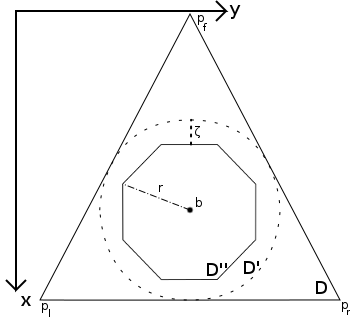
\includegraphics[width=4in]{ctr_base.png}
						\caption{Représentation des contraintes de non-basculement. $D$ correspond à la contrainte exacte.
							 $D'$ correspond à la contrainte circulaire inscrite dans $D$, rendant celle-ci invariante par rotation atour de $b$.
							 $D''$ correspond à la linéarisation de la contrainte $D'$ par un octogone, en ajoutant une marge de sécurité $\zeta$.}
						\label{fig.ctr_base2}
					}
				
				
					La contrainte principale à la stabilité de la commande est celle empêchant le robot de basculer \rfi{fig.ctr_base2}.
					Nous rappelons l'expression des contraintes de non-basculement \rf{eq.ctr_cop_1}\rf{eq.ctr_cop_2}\rf{eq.ctr_cop_3}.
					$\forall k \in (1, n)$ :
					\eqa{
						d^{xy}_k \times (p_r^{xy}-p_f^{xy}) &> 0 \\
						d^{xy}_k \times (p_l^{xy}-p_r^{xy}) &> 0 \\
						d^{xy}_k \times (p_f^{xy}-p_l^{xy}) &> 0
					}
					
					Ces contraintes ne sont pas invariantes par rotation de la base mobile.
					On réduit donc celles-ci à un cercle d'origine $B^{xy}$ que l'on linéarise par la suite par un octogone régulier de rayon $r'$, orienté selon la direction $\vec{x}$ \rfi{fig.ctr_base2}:
					\eqa{
						r' &= \min\prt{d_f, d_r, d_l} - \zeta  \\
						\zeta &>0
					}
					où $\zeta$ est une marge de sécurité. La formulation QP ne permet pas l'utilisation de contraintes d'inégalités strictes, la marge de sécurité $\zeta$ permet de s'en affranchir.
					
					Les contraintes linéarisées s'expriment donc directement de la façon suivante :
					\eq{
						v^-_1 \leq V_1X \leq v^+_1
					}
					avec
					\eqa{
					\nonumber
						V_1 &= \mat{
							U_{dc} & 0 & U_{db}-U_b & 0 \\
							0 & U_{dc} & 0 & U_{db}-U_b \\
							U_{dc} & U_{dc}  & U_{db}-U_b & U_{db}-U_b \\
							U_{dc} & -U_{dc}  & U_{db}-U_b & -U_{db}+U_b 
						}\\
					\nonumber
						v^-_1 &= \mat{
							-3\tilde{r}-S_{dc}\hat{c}^x-(S_{db}-U_b)\hat{b}^x \\
							-3\tilde{r}-S_{dc}\hat{c}^y-(S_{db}-U_b)\hat{b}^y \\
							-4\tilde{r}-S_{dc}(\hat{c}^x+\hat{c}^y)-(S_{db}-U_b)(\hat{b}^x+\hat{b}^y) \\
							-4\tilde{r}-S_{dc}(\hat{c}^x-\hat{c}^y)-(S_{db}-U_b)(\hat{b}^x-\hat{b}^y) 
						}\\
						v^+_1 &= \mat{
							3\tilde{r}-S_{dc}\hat{c}^x-(S_{db}-U_b)\hat{b}^x \\
							3\tilde{r}-S_{dc}\hat{c}^y-(S_{db}-U_b)\hat{b}^y \\
							4\tilde{r}-S_{dc}(\hat{c}^x+\hat{c}^y)-(S_{db}-U_b)(\hat{b}^x+\hat{b}^y) \\
							4\tilde{r}-S_{dc}(\hat{c}^x-\hat{c}^y)-(S_{db}-U_b)(\hat{b}^x-\hat{b}^y) 
						}
					}
					et $\tilde{r} = \dfrac{r'}{\sqrt{10}}$.
					
				
				\subsubsubsection{Vitesses et accélérations maximales de la base mobile}
				\label{section.ctr_base_3_roues}
				
				Les moteurs des roues de la base mobile sont limités en vitesse et accélération. Il faut donc prendre en compte cet élément afin de ne pas générer de commandes infaisables par le robot.
				Il n'y a pas de relation linéaire entre les limites cinématiques des moteurs des roues et celles de la base mobile.
				Nous allons donc définir des contraintes concernant la base mobile, conservatives vis à vis de celles des moteurs.
				
				Soit $\dot{b}_{m}$ et $\ddot{b}_{m}$ des limites en vitesse et accélération de la base mobile, nous pouvons exprimer les contraintes de la façon suivante.  
				$\forall k \in (1, n)$ :
				\eqa{
					\norm{\vec{\dot{b}}_k} &\leq \dot{b}_{m} \\
					\norm{\vec{\ddot{b}}_k} &\leq \ddot{b}_{m}
				}
				
				Ces contraintes étant non-linéaires, nous avons choisi de les approximer simplement par un carré, car, contrairement aux contraintes sur le CoP, celles-ci ne sont pas critiques concernant la stabilité du robot.
				Ainsi, même si les contraintes linéaires résultantes sont significativement non-conservatives par rotation du robot, cela n'impacte que de façon mineure le comportement de la commande.
				Cette solution est donc préférable, du point de vue du temps de calcul de la commande, au choix d'un polygone d'ordre plus élevé.
				
				
				Les contraintes linéarisées s'expriment donc de la façon suivante :
					\eq{
						v^-_2 \leq V_2X \leq v^+_2
					}
					avec :
					\eqa{
						V_2 &= \mat{
							0 & 0 & U_{\dot{b}} & 0 \\
							0 & 0 & 0 & U_{\dot{b}} \\
							0 & 0 & U_{\dot{b}} & 0 \\
							0 & 0 & 0 & U_{\dot{b}}
						},~~
						v^-_2 = \mat{
							-\tilde{\dot{b}}_m - S_{\dot{b}}\hat{b}^x \\
							-\tilde{\dot{b}}_m - S_{\dot{b}}\hat{b}^y \\
							-\tilde{\ddot{b}}_m - S_{\ddot{b}}\hat{b}^x \\
							-\tilde{\ddot{b}}_m - S_{\ddot{b}}\hat{b}^y \\
						},~~
						v^+_2 = \mat{
							\tilde{\dot{b}}_m - S_{\dot{b}}\hat{b}^x \\
							\tilde{\dot{b}}_m - S_{\dot{b}}\hat{b}^y \\
							\tilde{\ddot{b}}_m - S_{\ddot{b}}\hat{b}^x \\
							\tilde{\ddot{b}}_m - S_{\ddot{b}}\hat{b}^y \\
						}
					}
					et :
					\eqa{
						\tilde{\dot{b}}_m = \frac{\sqrt{2}}{2}\dot{b}_m \\
						\tilde{\ddot{b}}_m = \frac{\sqrt{2}}{2}\ddot{b}_m
					}
	
				
				\subsubsubsection{Limites articulaires du corps du robot}
				\label{section.ctr_body_3_roues}
			
					\fig{
						\centering
						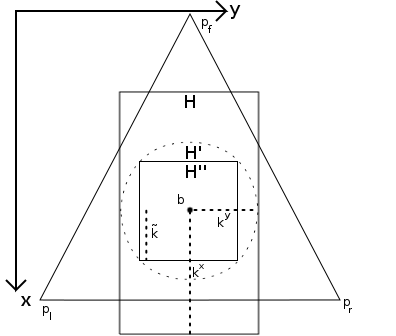
\includegraphics[width=4in]{ctr_body.png}
						\caption{Représentation des contraintes cinématiques du corps du robot. $H$ correspond à la contrainte exacte.
							 $H'$ correspond à la contrainte circulaire inscrite dans $H$, rendant celle-ci invariante par rotation autour de $b$.
							 $H''$ correspond à la linéarisation de la contrainte $H'$ par un carré.}
						\label{fig.ctr_body}
					}
					
					L'agencement des corps et articulations du robot implique que la distance entre son CoM $C^{xy}$ et celui de la base mobile $B^{xy}$ est limitée.
					Sur la plate-forme expérimentale, si l'on considère les approximations réalisées dans le chapitre \rf{chapitre.modele} ($c^z$ constant et on ignore les mouvements des bras),
					cette zone de déplacement correspond exactement à un rectangle centré autour de $B^{xy}$, de dimension $(2k^x, 2k^y)$ \rfi{fig.ctr_body}.
					
					Cette contrainte n'est pas invariante par rotation.
					Nous choisissons donc de réduire cette contrainte à un cercle centré autour de la base mobile $B^{xy}$, de rayon $\min\prt{k^x, k^y}$.
					Enfin, on linéarise ce cercle en un carré de dimension $2\tilde{k}$ \rfi{fig.ctr_body}, avec :
					\eq{
						\tilde{k} = \frac{\sqrt{2}}{2}\min\prt{k^x, k^y}
					}
					
					Nous ne choisissons pas ici un polygone d'ordre supérieur à $2$ car les limites articulaires du corps du robot sont dans la majorité des cas négligeables devant celles concernant le CoP.
					Ainsi, dans une situation normale, le robot ne se retrouve généralement pas en contrainte sur ses limites articulaires, ce qui rend un polygone d'ordre $2$ suffisant pour représenter les contraintes associées.
					
					Les contraintes linéarisées s'expriment donc de la façon suivante :
					\eq{
						v^-_3 \leq V_3X \leq v^+_3
					}
					avec
					\eqa{
						V_3 &= \mat{
							U_c & 0 & -U_b & 0 \\
							0 & U_c & 0 & -U_b
						},~~
						v^-_3 = \mat{
							-\tilde{k} - S_c\hat{c}^x + S_b\hat{b}^x \\
							-\tilde{k} - S_c\hat{c}^y + S_b\hat{b}^y
						},~~
						v^+_3 = \mat{
							\tilde{k} - S_c\hat{c}^x + S_b\hat{b}^x \\
							\tilde{k} - S_c\hat{c}^y + S_b\hat{b}^y
						}
					}
					
					

			\subsubsection{Problème quadratique résultant}
				\label{section.qp_3roues}
				
				La loi de commande optimale présentée possède plusieurs objectifs. Il existe classiquement deux manières de résoudre une problème multi-objectifs :
				\liste{
					\item Considérer une hiérarchie d'objectifs. A chaque niveau hiérarchique, un seul objectif est optimisé, ceux qui sont prioritaires sont considérés comme des contraintes, et les autres ne sont pas optimisés à ce niveau de hierarchie.
					\item Considérer une somme pondérée d'objectifs. Plus les pondérations associées sont relativement grandes les unes par rapport aux autres, plus les objectifs associés sont prioritaires.
				}
				
				Nous avons fait le choix de résoudre le problème par une somme pondérée d'objectifs. 
				Ce choix est motivé d'une part par le fait que les solveurs de QP que nous avions de disponibles ne permettent pas de résoudre un problème hiérarchique.
				D'autre part, en utilisant le principe d'une somme pondérée d'objectifs, nous pouvons tendre vers la première solution en augmentant l'écart relatif entre les pondérations de plusieurs ordres de grandeurs.
				Réaliser l'inverse n'est pas possible.
				
				Soit $\alpha_i$ la pondération associée à l'objectif $i$, nous pouvons écrire le problème quadratique résultant de la façon suivante :
				\eq{
					\lst{
						\min\limits_X \prt{\tr{X}\somme{i=1}{5}{\alpha_iQ_i}X+\somme{i=1}{5}{\alpha_i\tr{\rho}_i}X} \\
						\mat{v_1^- \\ v_2^- \\ v_3^-} \leq \mat{V_1 \\ V_2 \\ V_3} X \leq \mat{v_1^+ \\ v_2^+ \\ v_3^+}
					}
				}
				
				

		\subsection{Lorsque le robot bascule sur deux roues}
			\label{section.mpc_deux_roues}
			\subsubsection{Formulation des objectifs}
			
				Lorsque le robot bascule sur deux roues, nous pouvons définir trois objectifs de commande :
				\liste{
					\item Contrôler l'angle de basculement à $0$, afin de ramener le robot sur trois roues.
					\item Minimiser la vitesse angulaire de basculement. Cet objectif a pour but de limiter l'impact occasionné lorsque l'angle de basculement atteint $0$.
					      Si la vitesse angulaire est nulle au moment où la roue touche le sol, il n'y a pas d'impact.
					\item Assurer la stabilité numérique de la commande optimale. Cela peut être réalisé en minimisant le carré des variables de commande $X'$.
				}
				
				Dans la suite, nous noterons $O'_i$ l'objectif $i$. Il correspond à la norme élevée au carré d'une fonction des variables de commande. Il s'écrit de la façon suivante :
				\eq{
					O'_i = \frac{1}{2}\norm{f'_i(X)}^2
				}
				puis, en utilisant la notation QP :
				\eq{
					O'_i = \frac{1}{2}\tr{X}Q'_iX + \tr{\rho'}_iX + \epsilon'_i
				}
				avec $Q'_i$ une matrice symétrique définie positive (dite Hessienne), $\rho'_i$ un vecteur et $\epsilon_i$ un scalaire constant.
				Nous ne détaillerons pas l'expression des $\epsilon'_i$ car ce terme n'a pas d'impact pas dans la minimisation des l'objectifs $O'_i$.
				
				On rapelle le vecteur de commande dans le cas où le robot bascule sur deux roues :
				\eq{
					X' = \tr{\mat{\dddot{C}^n & \dddot{B}^n}}
				}
				
				\subsubsubsection{Minimisation de l'angle de basculement}
				
					L'objectif principal de la commande est d'assurer le retour sur trois roues au sol du robot en amenant l'angle de basculement à $0$.
					Nous pouvons donc écrire l'objectif $O'_1$ correspondant en utilisant l'équation \rf{eq.dyn_tilt_pred} :
					\eq{
						O'_1 = \frac{1}{2}\norm{\Psi}^2 = \frac{1}{2}\tr{X'}Q'_1X'+\tr{\rho'}_1X+\epsilon'_1
					}
					avec :
					\eqa{
					\nonumber
						Q'_1 &= \mat{
							\tr{U}_{\psi c}\tilde{U}^{-t}_{\psi}\tilde{U}^{-1}_{\psi}U_{\psi c} & \tr{U}_{\psi c}\tilde{U}^{-t}_{\psi}\tilde{U}^{-1}_{\psi}U_{\psi b} \\
							\tr{U}_{\psi b}\tilde{U}^{-t}_{\psi}\tilde{U}^{-1}_{\psi}U_{\psi c} & \tr{U}_{\psi b}\tilde{U}^{-t}_{\psi}\tilde{U}^{-1}_{\psi}U_{\psi b}	
						}\\
						\rho'_1 &= \mat{
							\tr{U}_{\psi c}\tilde{U}^{-t}_{\psi}(S_{\psi b}\hat{b}^n + S_{\psi c}\hat{c}^n + S_{\psi g^x}g^x + S_{\psi g^y} g^y + S_{\psi \psi} \hat{\psi}) \\
							\tr{U}_{\psi b}\tilde{U}^{-t}_{\psi}(S_{\psi b}\hat{b}^n + S_{\psi c}\hat{c}^n + S_{\psi g^x}g^x + S_{\psi g^y} g^y + S_{\psi \psi} \hat{\psi})
						}
					}
				
				\subsubsubsection{Minimisation de la vitesse angulaire}
				
					Afin de limiter l'impact du robot lorsqu'il touchera le sol, il est important de minimiser la vitesse angulaire de basculement.
					Pour exprimer l'objectif correspondant, il faut dans un premier temps écrire les relations entre la vitesse angulaire de basculement $\dot{\Psi}$ et les variables du problème $X'$.
					\eq{
						\dot{\Psi} = U_{\dot{\psi}}\dddot{\Psi} + S_{\dot{\psi}}\hat{\psi}
					}
					
					En utilisant l'équation \rf{eq.dyn_tilt_pred}, on peut donc écrire :
					\eq{
					\label{eq.dot_psi}
						\dot{\Psi} = U_{\dot{\psi}}\tilde{U}^{-1}_\psi \prt{U_{\psi b}\dddot{B}^n + U_{\psi c}\dddot{C}^n + S_{\psi b}\hat{b}^n 
						           + S_{\psi c}\hat{c}^n + S_{\psi g^x}g^x + S_{\psi g^y} g^y} + \prt{U_{\dot{\psi}} \tilde{U}^{-1}_\psi  S_{\psi \psi} + S_{\dot{\psi}}} \hat{\psi}
					}

					Nous pouvons donc écrire l'objectif $O'_2$ : 
					\eq{
						O'_2 = \frac{1}{2}\norm{\dot{\Psi}}^2 = \frac{1}{2}\tr{X'}Q'_2X'+\tr{\rho'}_2X+\epsilon'_2
					}
					avec :
					\eqa{
						\nonumber	
						Q'_2 &= \mat{
							\tr{U}_{\psi c}\tilde{U}^{-t}_\psi\tr{U_{\dot{\psi}}} U_{\dot{\psi}}\tilde{U}^{-1}_\psi U_{\psi c} & \tr{U}_{\psi c}\tilde{U}^{-t}_\psi\tr{U_{\dot{\psi}}} U_{\dot{\psi}}\tilde{U}^{-1}_\psi U_{\psi b} \\
							\tr{U}_{\psi b}\tilde{U}^{-t}_\psi\tr{U_{\dot{\psi}}} U_{\dot{\psi}}\tilde{U}^{-1}_\psi U_{\psi c} & \tr{U}_{\psi b}\tilde{U}^{-t}_\psi\tr{U_{\dot{\psi}}} U_{\dot{\psi}}\tilde{U}^{-1}_\psi U_{\psi b}  
						}\\
						\rho'_2 &= \mat{
							\tr{U}_{\psi c}\tilde{U}^{-t}_\psi\tr{U_{\dot{\psi}}} \prt{U_{\dot{\psi}}\tilde{U}^{-1}_\psi (S_{\psi b}\hat{b}^n + S_{\psi c}\hat{c}^n + S_{\psi g^x}g^x + S_{\psi g^y} g^y) + (U_{\dot{\psi}} \tilde{U}^{-1}_\psi  S_{\psi \psi} + S_{\dot{\psi}}) \hat{\psi}} \\
							\tr{U}_{\psi b}\tilde{U}^{-t}_\psi\tr{U_{\dot{\psi}}} \prt{U_{\dot{\psi}}\tilde{U}^{-1}_\psi (S_{\psi b}\hat{b}^n + S_{\psi c}\hat{c}^n + S_{\psi g^x}g^x + S_{\psi g^y} g^y) + (U_{\dot{\psi}} \tilde{U}^{-1}_\psi  S_{\psi \psi} + S_{\dot{\psi}}) \hat{\psi}} 
						}
					}
				
				\subsubsubsection{Stabilité numérique}
				
					Le dernier objectif concerne la stabilité numérique du problème d'optimisation.
					Afin de réaliser cela, une solution consiste à minimiser le jerk des commandes $\dddot{C}^{n}$ et $\dddot{B}^{n}$.
					
					Nous pouvons donc écrire le dernier objectif $O'_5$ :
					\eq{
						O'_3 = \frac{1}{2}\norm{X'}^2 = \frac{1}{2}\tr{X}Q'_3X + \tr{\rho'}_3X + \epsilon_3
					}
					avec : 
					\eq{
						Q'_3 = \id, ~~\rho'_3 = 0
					}

			\subsubsection{Formulation des contraintes}
			
				Lorsque le robot est en basculement sur deux roues, il est important de définir un certain nombre de contraintes :
				\liste{
					\item Respecter les contraintes de non-pénétrtation dans le sol, en assurant que l'angle de basculement $\Psi$ est toujours positif ou nul.
					\item Respecter les limites physiques de la base mobile en limitant les vitesses et accélérations maximales
					\item Respecter la cinématique du corps du robot, en limitant la distance entre son CoM $C^{xy}$ et celui de la base mobile $B^{xy}$.
				}
				
				Contrairement à la section \rf{ctr_intro_3_roues}, le robot ne peut pas tourner pendant le contrôle du basculement ($B^t$ et $C^t$ constant).
				Il n'est donc pas nécessaire de rendre les contraintes invariantes par rotation autour de la base $B$.
				
				Dans les sections suivantes, nous écrirons les contraintes linéarisées de la façon suivante :
				\eq{
					v'^-_i \leq V'_iX' \leq v'^+_i
				}
				
				\subsubsubsection{Contraintes de non-pénétration dans le sol}
				
					La présence du sol fait que l'angle de basculement $\Phi$ ne peut pas etre négatif.
					Cette contrainte est directement linéaire en les variables de commande et s'exprime ainsi :
					\eq{
						\Phi \ge 0
					}
					
					On peut donc écrire la contrainte de la façon standard :
					\eq{
						v'^-_1 \leq V'_1X' \leq v'^+_1
					}
					avec :
					\eqa{
					\nonumber
						V'_1 &= \mat{
							\tilde{U}^{-1}U_{\psi c} & \tilde{U}^{-1}U_{\psi b}
						} \\
					\nonumber
						v'^-_1 &= \mat{
							-\tilde{U}^{-1}\prt{S_{\psi b}\hat{b}^n + S_{\psi c}\hat{c}^n + S_{\psi g^x}g^x + S_{\psi g^y} g^y + S_{\psi \psi} \hat{\psi}}
						}\\
						v'^+_1 &= \mat{
							+\infty
						}
					}
				
				\subsubsubsection{Vitesses et accélérations maximales de la base mobile}
				
					De façon identique à la section \rf{section.ctr_base_3_roues}, les contraintes en vitesse et accélération de la base mobile s'écrivent de la façon suivante :	
					\eqa{
						\norm{\vec{\dot{b}}_k} &\leq \dot{b}_{m} \\
						\norm{\vec{\ddot{b}}_k} &\leq \ddot{b}_{m}
					}
					
					Le robot ne pouvant se déplacer qu'uniquement sur la droite représentée par le vecteur $\vec{n}_k$, les contraintes peuvent se réécrire de la façon suivante :
					\eqa{
						\dot{b}^n &\leq \dot{b}_{m} \\
						\ddot{b}^n &\leq \ddot{b}_{m} 
					}
					ce qui se réécrit de façon standard :
					\eq{
						v'^-_2 \leq V'_2X' \leq v'^+_2
					}
					avec :
					\eq{
						V'_2 = \mat{
							0 & U_{\dot{b}} \\
							0 & U_{\ddot{b}} \\
						},~~
						v'^-_2 = \mat{
							-\dot{b}_{m} - S_{\dot{b}}\hat{b}^n \\
							-\ddot{b}_{m} - S_{\ddot{b}}\hat{b}^n \\
						},~~
						v'^+_2 = \mat{
							\dot{b}_{m} - S_{\dot{b}}\hat{b}^n \\
							\ddot{b}_{m} - S_{\ddot{b}}\hat{b}^n \\
						}
					}					
				
				\subsubsubsection{Limites articulaires du corps du robot}
				
					\fig{
						\centering
						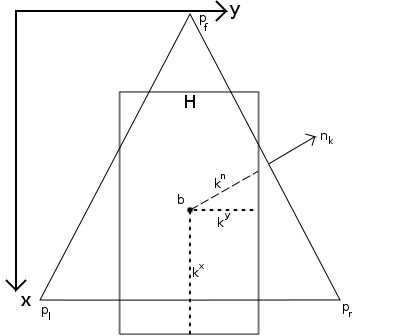
\includegraphics[width=4in]{ctr_body_tilt.png}
						\caption{Représentation des contraintes cinématiques du corps du robot lorsque celui-ci bascule. $H$ correspond à la contrainte exacte. 
						         $k^n$ correspond à la distance entre le point $b$ et le point d'intersection de l'axe $(b, \vec{n}_k)$ et l'enveloppe $H$}
						\label{fig.ctr_body_tilt}
					}
					
					De façon identique à la section \rf{section.ctr_body_3_roues}, on défini la contrainte entre le CoM du corps du robot $C$ et celui de la base mobile $B$ par un rectangle de dimensions $(k^x, k^y)$ centré en $b$.
					
					Soit $k^n$ la distance du segment reliant le centre de la base mobile $B$ et le point d'intersection entre la droite définie par le vecteur $\vec{n}_k$ et d'origine $B$ avec le rectangle de la contrainte. $k^n$ s'exprime de la façon suivante \rfi{fig.ctr_body_tilt} :
					\eq{
						k^n = \min\prt{
							\norm{k^x\cos(\theta_k)},
							\norm{k^y\sin(\theta_k)}
						}
					}
					
					La contrainte s'exprime de la façon suivante :
					\eq{
						-k^n \leq C^n-B^n \leq k^n
					}
					ce qui se réécrit de façon standard :
					\eq{
						v'^-_3 \leq V'_3X' \leq v'^+_3
					}
					avec :
					\eqa{
						V'_3 = \mat{
							U_c & -U_b
						},~~
						v'^-_3 = \mat{
							-k^n - S_c\hat{c}^n + S_b\hat{b}^n
						},~~
						v'^+_3 = \mat{
							k^n - S_c\hat{c}^n + S_b\hat{b}^n
						}
					}

			\subsubsection{Problème quadratique résultant}
		
				De la même manière qu'en section \rf{section.qp_3roues}, nous pouvons écrire le problème quadratique résultant de la façon suivante :
				\eq{
					\lst{
						\min\limits_{X'} \prt{\tr{X'}\somme{i=1}{3}{\alpha'_iQ'_i}X'+\somme{i=1}{3}{\alpha'_i\tr{\rho'}_i}X'} \\
						\mat{v'^-_1 \\ v'^-_2 \\ v'^-_3} \leq \mat{V'_1 \\ V'_2 \\ V'_3} X \leq \mat{v'^+_1 \\ v'^+_2 \\ v'^+_3}
					}
				}
				avec $\alpha'_i$ la pondération associée à l'objectif $O'_i$.

		\subsection{Gestion de la transition entre les deux états}
		\label{section.mpc_transition}
		
			Le contrôleur décrit en section \rf{section.mpc_deux_roues} ne prend pas en compte la force de réaction qui se rajoute au moment où l'angle de basculement atteint $0$.
			Cela amène ce contrôleur à générer une très grande accélération afin de maintenir l'angle à $0$. 
			Bien que celle-ci puisse être réalisable, ce comportement n'est pas souhaitable et nous préférons ``laisser tomber'' le robot sur le sol lorsque celui-ci va le percuter, afin d'éviter un déplacement exagéré de la base mobile.
			
			Il faut donc adjoindre aux deux précédents contrôleurs un troisième permettant de gérer cet état. Nous choisissons d'utiliser le jeu de variable $X$.
			Les objectifs choisis sont :
			\liste{
				\item $O_3$ et $O_4$. Contrôler le CoP au milieu de la base en utilisant le modèle de robot sur trois roues permet d'assurer au robot de ne pas accroitre son angle de basculement.
				      Cet objectif permet de contrôler le moment angulaire du robot autour de son axe de rotation afin qu'il soit toujours dirigé vers la bonne direction, lorsque celui-ci est proche du sol.
				\item $O_5$. Assurer la stabilité numérique de l'algorithme est toujours indispensable.
			}
			
			Les contraintes choisies sont :
			\liste{
				\item $(V_1, v^+_1, v^-_1)$. La contrainte sur le CoP permet d'assurer au robot que son moment angulaire va faire tomber celui-dernier sur ces trois roues, lorsque celui-ci est  proche du sol.
				\item $(V_2, v^+_2, v^-_2)$ et $(V_3, v^+_3, v^-_3)$. Afin de ne pas générer de mouvements infaisables, il faut contraindre le déplacement de la base mobile et du corps du robot.
			}
			
			Il faut cependant prendre en compte que le robot est toujours sous-actionné, car ayant une roue en l'air. 
			Il s'impose donc de rajouter une contrainte concernant le déplacement de la base mobile, qui doit se faire uniquement selon l'axe $\vec{n}_k$.
			Cette contrainte s'exprime de la façon suivante :
			\eq{
				\cos(\theta_k)\dot{B}^y = \sin(\theta_k)\dot{B}^x
			}
			ce qui se réécrit de façon standard :
					\eq{
						v^-_4 \leq V_4X \leq v^+_4
					}
					avec :
					\eqa{
					\nonumber
						V_4 &= \mat{
							0 & 0 & \sin(\theta_k)U_{\dot{b}} & - \cos(\theta_k)U_{\dot{b}}
						}\\
						v^-_4 &= v^+_4 = \mat{
							\cos(\theta_k)S_{\dot{b}}\hat{b}^y - \sin(\theta_k)S_{\dot{b}}\hat{b}^x
						}
					}

			Le problème quadratique résultant s'écrit donc :
			\eq{
				\lst{
					\min\limits_{X} \prt{\tr{X}\somme{i=3}{5}{\alpha_iQ_i}X'+\somme{i=3}{5}{\alpha_i\tr{\rho}_i}X} \\
					\mat{v^-_1 \\ v^-_2 \\ v^-_3 \\ v^-_4} \leq \mat{V_1 \\ V_2 \\ V_3 \\ V_4} X \leq \mat{v^+_1 \\ v^+_2 \\ v^+_3 \\ v^+_4}
				}
			}
			

	\section{Gestion des deux modèles dynamiques exclusifs}
		\label{section.superviseur}
		\subsection{Choix d'un superviseur et conséquences}
		
			L'objectif est maintenant de définir un moyen permettant de choisir quel contrôleur parmi les trois proposés en sections \rf{section.mpc_trois_roues}\rf{section.mpc_deux_roues}\rf{section.mpc_transition} doit être activé afin de commander le robot.
			Nous avons fait le choix d'un superviseur basé sur une machine a états et d'une heuristique de transition entre ces états.
		
			Les avantages de ce type de superviseur sont qu'il est facile à implémenter ainsi qu'à en faire évoluer les paramètres associés aux heuristiques de transition.
			De plus, ce type de superviseur permet de gérer de façon simple les transitions de modes dynamiques ainsi que les impacts.
			
			Les inconvénient sont le fait que l'utilisation d'heuristiques rend le comportement du robot non-optimal à une situation donné.
			De plus, si celles-ci sont mal choisies, son comportement peut être contraire aux objectifs de commande et impacter négativement son équilibre. 
			Nous verrons notament les conséquences de l'utilisation d'heuristiques de transitions au chapitre \rf{chapitre.resultats}
			
			Dans la suite, il est important de prendre en compte au fait que certaines heuristiques ont été faites pour prendre en compte les perturbations les plus communes qu'un humain peut appliquer à la plate-forme expérimentale.
			
		\subsection{Fonctionnement du superviseur}

			\fig{
				\centering
				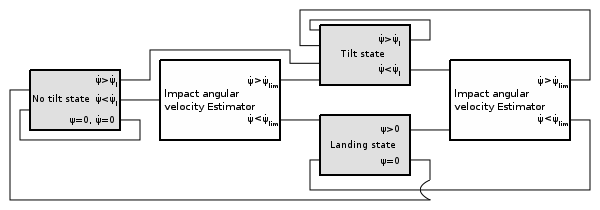
\includegraphics[width=6.5in]{supervisor.png}
				\caption{Schéma de fonctionnement du superviseur. 
					Les boites ``No tilt state'', ``Tilt state'' et ``Landing state'' correspondent aux états du superviseur.
					Les boites ``impact angular velocity estimator'' correspondent à l'estimateur de vitesse d'impact, permettant de gérer la transition entre les états.}
				\label{fig.supervisor}
			}
			
			\subsubsection{Les états du superviseur}
				
				
				La machine à états du superviseur est composé de trois états \rfi{fig.supervisor} :
				\liste{
					\item L'état \textit{No tilt} indique que le robot possède les trois roues sur le sol. Le contrôleur développé en section \rf{section.mpc_trois_roues} est donc activé.
					\item L'état \textit{Tilt} indique que le robot est en basculement sur deux roues. Le contrôleur développé en section \rf{section.mpc_deux_roues} est donc activé.
					\item l'état \textit{Landing} indique que le robot est en basculement sur deux roues, mais proche du sol et sur le point de le toucher. Le contrôleur développé en section \rf{section.mpc_transition} est donc activé.
				}
				
				Afin de définir les transitions entre les états, trois mesures sont utilisées : l'angle de basculement, la vitesse angulaire, et l'estimation de la vitesse angulaire d'impact.
			
			\subsubsection{Les transitions depuis l'état \textit{No tilt}}
			
				Lorsque le superviseur est dans l'état \textit{No tilt}, les transitions sont les suivantes \rfi{fig.supervisor} :
				\liste{
					\item Si la vitesse angulaire mesurée est supérieure à une limite donnée $\psi_l$, alors le superviseur passe à l'état \textit{Tilt}. 
					On ne peut pas prévoir la durée ni l'intensité de la perturbation dans le futur.
					Ainsi, si on mesure une forte vitesse angulaire, on suppose que l'humain qui pousse le robot ne va pas arrêter son geste rapidement, au moins pour des raisons d'inertie.
					
					\item Si la vitesse angulaire est inférieure à $\psi_l$, mais non-nulle, on utilise un estimateur de vitesse angulaire d'impact (qui sera décrit en section \rf{section.impact_estimator}).
					Si celui-ci indique que, sans compensation active par le contrôleur \rf{section.mpc_deux_roues}, le robot va tomber ou avoir une trop grande vitesse angulaire estimée au moment de l'impact, alors le superviseur passe à l'état \textit{Tilt}.
					Cet estimateur permet de déterminer si le robot va tomber, en considérant un arrêt de la force de perturbation et une absence de compensation par le contrôleur \rf{section.mpc_deux_roues}.
					Si non, cet estimateur indique la vitesse angulaire d'impact.
					
					\item Dans le cas où l'estimateur indique que la vitesse angulaire d'impact estimée est suffisamment faible, alors le superviseur passe à l'état \textit{Landing}.
					Cela signifie que le robot va compenser passivement la perturbation et ne pas générer un impact trop élevé. 
					Dans ce cas, le mieux est de stopper le suivi de trajectoire, ainsi que de limiter le déplacement du robot dans l'axe de basculement, ce qui correspond bien au contrôleur de l'état \textit{Landing}.
					
					\item Dans tout les autres cas, le superviseur reste dans l'état \textit{No tilt}, car il n'est pas en train de basculer.
				}
				
			\subsubsection{Les transitions depuis l'état \textit{Tilt}}
			
				Lorsque le superviseur est dans l'état \textit{Tilt}, les transitions sont les suivantes  \rfi{fig.supervisor} :
				\liste{
					\item Si la vitesse angulaire mesurée est supérieure à $\psi_l$, alors le superviseur reste dans l'état \textit{Tilt}. 
					      Cela signifie que la perturbation n'a toujours pas été contrôlée.
					\item Dans le cas contraire, on utilise l'estimateur afin de déterminer la vitesse angulaire d'impact. 
					      Si celle-ci est trop forte, alors le superviseur reste dans l'état \textit{Tilt}.
					\item Dans le cas contraire, le superviseur passe à l'état \textit{Landing}.
					      Cela signifie que la perturbation a été suffisamment compensée pour à présent laisser tomber le robot sur le sol et finir de compenser passivement la perturbation.
				}
			
			\subsubsection{Les transitions depuis l'état \textit{Landing}}
			
				Lorsque le superviseur est dans l'état \textit{Landing}, les transitions sont les suivantes  \rfi{fig.supervisor} :
				\liste{
					\item Lorsque la vitesse angulaire et l'angle de basculement atteind $0$, après une légère période de temporisation afin d'éviter tout rebond éventuel, le superviseur passe à l'état \textit{No tilt}.
					\item Dans le cas contraire, on utilise l'estimateur afin de déterminer la vitesse angulaire d'impact. Si celle-ci est trop grande, alors le superviseur passe à l'état \textit{Tilt}.
					\item Dans le cas contraire, alors la phase atterrissage n'est pas terminée et le superviseur reste dans l'état \textit{Landing}.
				}
			

		\subsection{Fonctionnement de l'estimateur d'impact}
		\label{section.impact_estimator}

			Le premier objectif de l'estimateur d'impact est de déterminer si le robot va pouvoir compenser passivement la perturbation, ou bien tomber.
			Le second objectif est, dans le cas où le robot va pouvoir compenser passivement la perturbation, estimer la vitesse angulaire au moment de l'impact.
			
			L'estimateur utilise l'observation courante de l'angle de basculement ainsi que la mesure de la vitesse angulaire.
			On suppose dans un premier temps que le robot a une accélération angulaire constante dépendant uniquement de la gravité et de l'angle actuel de basculement :
			\eq{
			\label{eq.ddot_psi_estimateur}
				\ddot{\psi} = -\frac{g^z}{h_b}\cos\prt{\psi_0+$atan$\prt{\dfrac{h_b}{d_k}}}
			}
			
			A l'aide de l'équation \rf{eq.ddot_psi_estimateur}, on peut écrire l'évolution de l'angle de basculement au cours du temps :
			\eq{
				\psi = -\frac{g^z\cos\prt{\psi_0+$atan$\prt{\dfrac{h_b}{d_k}}}}{2h_b}t^2+\dot{\psi}_0t+\psi_0
			}
			
			En résolvant l'équation quadratique associée, pour $\psi=0$, on peut déterminer si le robot va impacter le sol, et si oui, estimer quel va être la vitesse angulaire d'impact.
			Soit $\Delta$ tel que :
			\eq{
				\Delta = \dot{\psi}_0^2+\dfrac{2g^z\psi_0\cos\prt{\psi_0+$atan$\prt{\dfrac{h_b}{d_k}}}}{h_b}
			}
			
			Si $\Delta<0$, le robot va tomber et il n'y aura pas d'impact de la roue en l'air sur le sol.
			Dans le cas contraire, le temps d'impact $t_i$ est calculé de la manière suivante :
			\eq{
				t_i = \dfrac{h_b(\dot{\psi}_0\pm \sqrt{\Delta})}{g^z\cos\prt{\psi_0+$atan$\prt{\dfrac{h_b}{d_k}}}}
			}
			et la vitesse d'impact estimée $\dot{\psi}_i$ est :
			\eq{
				\dot{\psi}_i = -\sqrt{\Delta}
			}

	\section{Vers une modélisation unifiée des deux dynamiques}
	\label{section.modelisation_unifiee}
	
		Dans cette section, nous présentons une méthode de résolution du problème d'unification des deux modèles dynamiques \rf{eq.dyn_cop_pred}\rf{eq.dyn_tilt_pred}.
		nous n'avons pas eu le temps d'implémenter cette méthode sur la plate-forme expérimentale, nous allons donc apporter uniquement un début d'approche théorique.
		
		Afin d'unifier les deux modèles dynamiques en un seul contrôleur, tout en restant dans le formalisme de la programmation quadratique linéaire, 
		une solution est de résoudre \textit{a priori} le problème d'optimisation sur l'ensemble de l'horizon de prédiction.
		Nous proposons l'heuristique suivante :
		\liste{
			\item 	Dans le cas où le robot possède initialement les trois roues en contact avec le sol, on considère que celui-ci le restera durant tout l'horizon de prédiction. 
				La loi de commande utilisée est directement celle présentée en section \rf{section.mpc_trois_roues}.
			\item 	Dans le cas où le robot est initialement en basculement sur deux roues (suite à une forte perturbation par exemple), on considère que celui-ci le restera sur l'intervalle $[0, m]$ de l'horizon de prédiction, où $m\leq n$.
				La loi de commande utilisée sur cet intervalle est de la forme de celle présentée en section \rf{section.mpc_deux_roues}
				Sur l'intervalle  $[m+1, n]$, si celui-ci existe ($m<n$), on considère que le robot est revenue sur ses trois roues.
				La loi de commande utilisée sur cet intervalle est de la forme de celle présentée en section \rf{section.mpc_trois_roues}.	
		}
		
		Cette heuristique implique notament le fait que lorsque le robot est en basculement sur deux roues, celui-ci va soit le rester durant tout l'horizon, soit retomber sans rebondir à l'instant $m$. 
		Cela est théoriquement pris en compte par les contraintes sur le CoP sur l'intervalle $[m+1, n]$, assurant au robot de ne pas rebondir.
		Il faut pour cela intégrer dans la formulation du CoP sur les instants $[m+1, n]$ l'influence de la vitesse et de l'accélération angulaire d'impact sur la formulation du CoP.
		
		De plus, une prédiction de la valeur de $m$ doit être faite. 
		Il faut donc, en s'inspirant de l'estimateur d'impact par exemple \rf{section.impact_estimator}, prédire cet instant $m$ et s'assurer qu'il converge vers la véritable valeur au fur et à mesure que $m$ tend vers $0$.
		
		Enfin, un travail de réécriture de la dynamique future doit être faite, de façon analogue à ce qui a été fait en section \rf{section.modele_futur}, afin de prendre en compte les deux modèles, ainsi que de leur transition entre les instants $m$ et $m+1$.
		
		
	\section{Conclusion}
	
		Dans ce chapitre, nous avons présenté une loi de commande composite permettant de contrôler l'équilibre et les mouvements d'un robot humanoïde à roues omnidirectionnelles.
		Celle-ci se base sur trois sous-lois de commandes optimales utilisant le formalisme de la programmation quadratique et supervisées par une machine a état.
		Ces trois lois permettent de contrôler le robot dans des situations différentes :
		\liste{
			\item Lorsque le robot est en contact sur le sol avec ces trois roues.
			\item Lorsque le robot bascule sur deux roues.
			\item Lorsque le robot va impacter le sol.
		}
		En estimant l'existence et la vitesse angulaire future d'impact du robot avec le sol, ainsi qu'en mesurant l'angle de basculement courant et sa vitesse angulaire, le superviseur est capable de choisir quelle sous-loi de commande activer à chaque instant.
		
		Enfin, l'ébauche d'une approche unifiée de cette loi de commande a été présentée afin de se passer de l'utilisation d'un superviseur, ainsi que d'améliorer la gestion de la transition entre les deux modes dynamiques (trois ou deux roues en contact avec le sol).
		
		
		